\section{Distinguish Hardware}\label{Sec:DistinguishDevice}
%Basic idea of this attack
IoT applications utilise a great variation of devices, with each having different processing power. Consequently, the time required for a specific operation could be exploited as an indicator to the hardware. 

The time required to process a PING Request could therefore be exploited to perform such hardware distinguishing attack. Although the same attack could be conducted on various packets, PING is specifically practical and ideal due to:
\begin{enumerate}
	\item PING is processed in a highly predictable manner where nearly no computation is required; thus minimises the noise induced by data dependency.
	\item Support to PING is mandatory according to the standard\cite{rfc4443}, making the attack universally applicable.
\end{enumerate}

For our experiments, the PING Requests are initiated from a Linux machine connected into the 6LoWPAN through a border router. The ``-s 0'' option is specified for the `ping6' command in order to avoid exceeding the MTU of 6LoWPAN (127 bytes). 

\subsection{Computing PING Response Time}\label{TimingWithContikiMAC}
%How to process the packets
%ContikiMAC
For energy preservation, Contiki adopts a Radio Duty Cycle (RDC) protocol called Contiki MAC\cite{ContikiMAC}. On receiver's side, Contiki MAC switches off the radio for most of the times and periodically wakes up for a short period for signal detection. If a signal is detected during the awaken period, the radio is kept on to receive a packet, followed by an acknowledgement sent to inform the sender. On sender's side, a packet is repeatedly transmitted until timed out or an acknowledgement is received.

Therefore when ContikiMAC is enabled by default, duplicated packets may be observed in the captured traffic. As an approximation to the PING Request processing time, we define PING Response Interval (PRI) as the time elapsed between the last PING Request and the first PING Response.

\begin{example}
%\paragraph{Example}

\AddFigure{fig/PRI.png}{PRI Example}{PRIExample}

\Cref{PRIExample} shows an example of packets captured by Wireshark\cite{Wireshark}. Duplicated PING Requests, No.$198$ to No.$203$, are replied by a single PING Response, No.$205$, matched by their \textit{seq} field ($16$). The PRI is therefore computed as the difference in time between No.$203$ (last PING Request) and No.$205$ (first PING Response) which is:
\begin{equation*}
PRI = 4.701468 - 4.684369 = 0.017099(s) = 17.099(ms)
\end{equation*}
\end{example}

\subsection{PRIs of TelosB and CC2538} \label{PRI_Devices}

\Cref{PRIs} shows the distributions of PRI collected on TelosB and CC2538. The bar on the right most represents the outliers in the data, with $9.43\%$ on TelosB are $\geq 19$ms and $2.60\%$ on CC2538 $\geq 12$ms respectively. 

The result of \Cref{PRIs} suggests that TelosB and CC2538 can be easily distinguished by their PRIs, as they are tightly clustered around $17$ms for TelosB and $9.5$ms for CC2538 respectively.

\begin{figure}[ht!]
	\centering
	\begin{subfigure}{0.45\linewidth}
		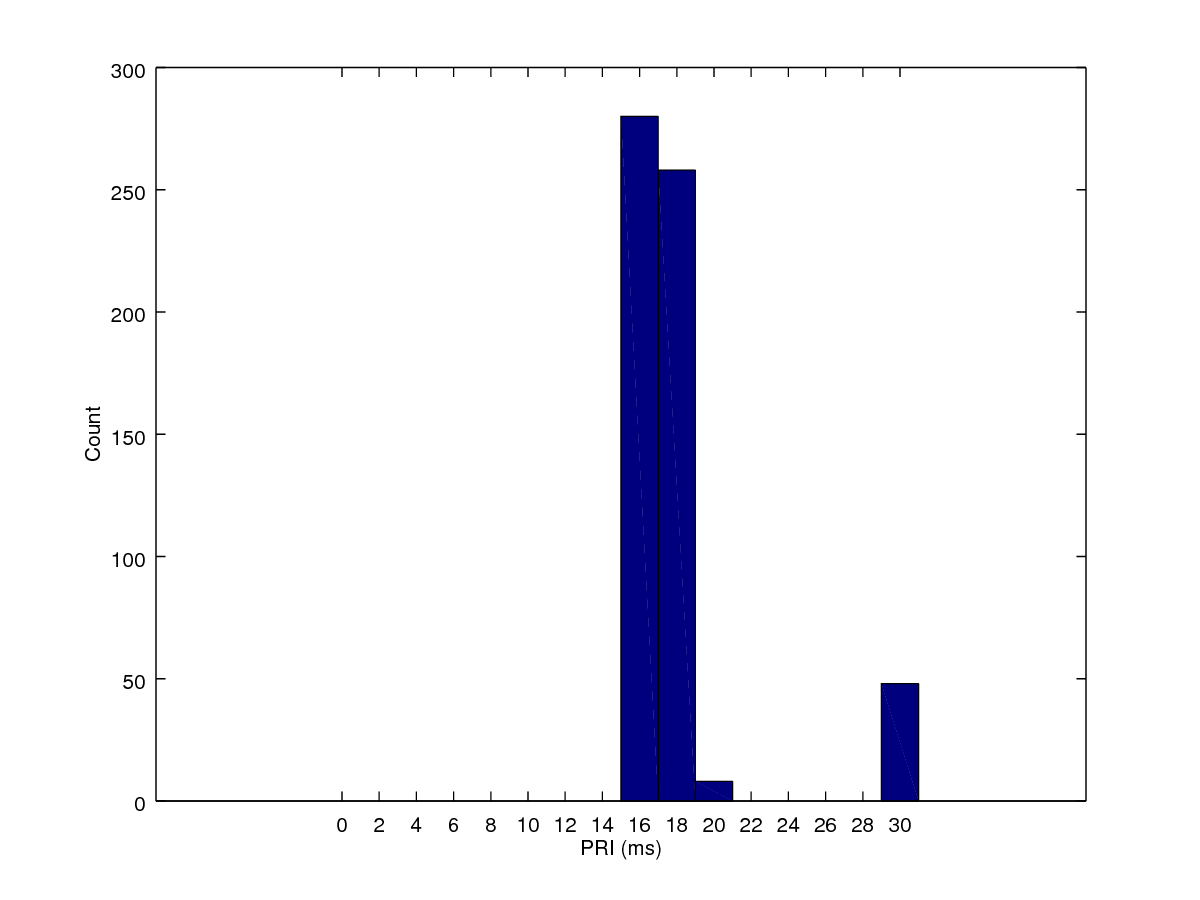
\includegraphics[width=\linewidth]{fig/helloworld_sky.png}
		\subcaption{TelosB PRIs}
	\end{subfigure}
	\begin{subfigure}{0.45\linewidth}
		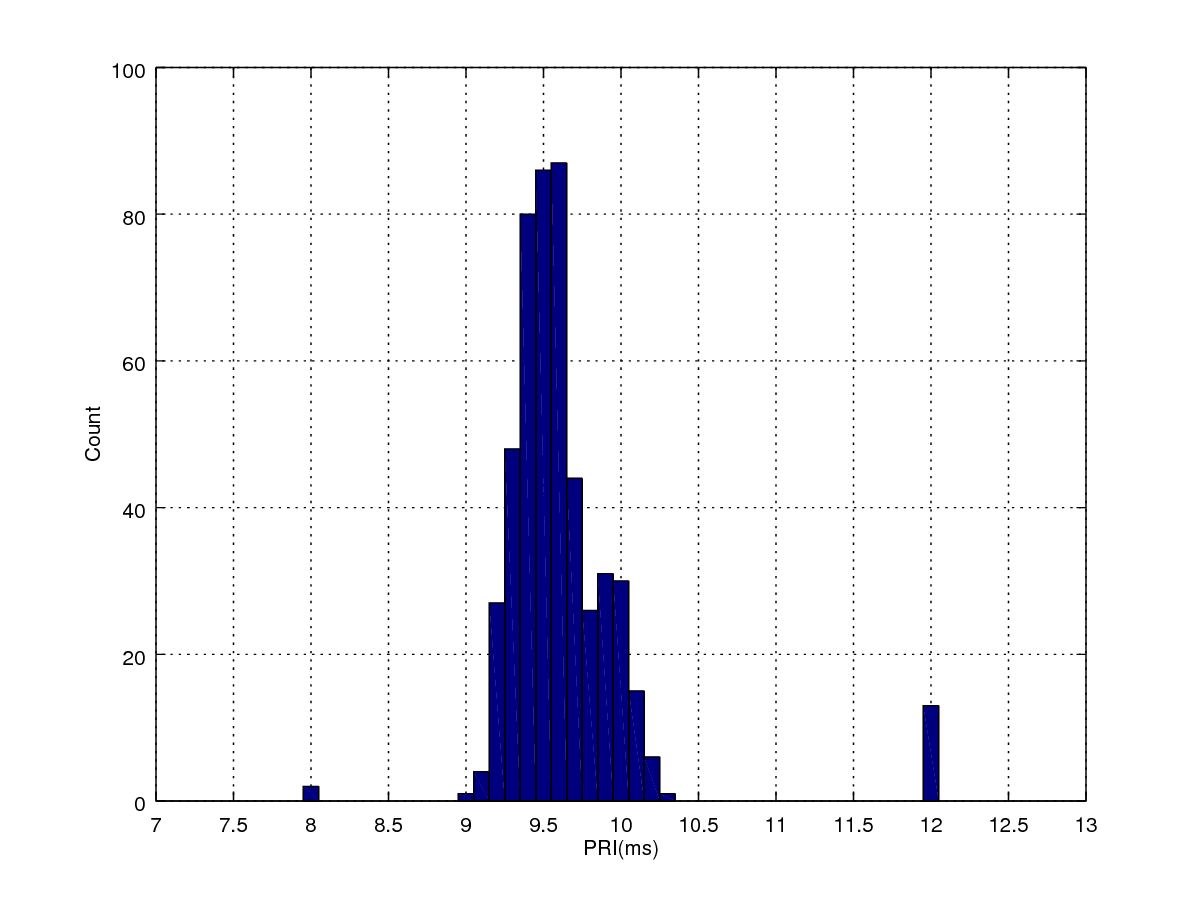
\includegraphics[width=\linewidth]{fig/helloworld_cc2538.png}
		\subcaption{CC2538 PRIs}
	\end{subfigure}
	
	\adjustbox{max width = \textwidth}
	{
		\begin{tabular}{|c|c|c|}
			\hline
			              & Mean (ms)     & Median (ms)   \\ \hline
			TelosB  & 33.82 & 17.03 \\ \hline
			CC2538 & 14.27         & 9.56          \\ \hline
		\end{tabular}
	}
	\caption{PRIs for different devices. \label{PRIs}}
\end{figure}

With respect to the outliers, one common cause is the processor being occupied by other tasks when a PING Request is received; thus delayed the processing of PING as illustrated by \Cref{PingProbeExample}. The portion of the outlier is hence affected by the payload on the node and the frequency of PING requests. We discuss further details of the outliers in \Cref{PingProbe}.

\AddFigure{fig/PingProbe_Session.png}{PRI prolonged by Sensor Reading}{PingProbeExample}

\subsection{Factors Affecting PRI} \label{PingDevice}

Despite the clear distinguishability suggested by \Cref{PRI_Devices}, there exists several practical factors the might affect the result.

802.15.4 Security\cite{802154} is a prominent factor to PRIs as it induces several cryptographic operations which are computationally heavy and hence could significantly increase the PRI. \Cref{802154SecPRI} illustrates the PRIs on the same devices when 802.15.4 Security is enabled. Flooding PING could also make an impact on measuring PRIs as it will overrun the low processing power of these resource constrained devices.

\begin{figure}[ht!]
	\centering
	\begin{subfigure}{0.4\textwidth}
	{
		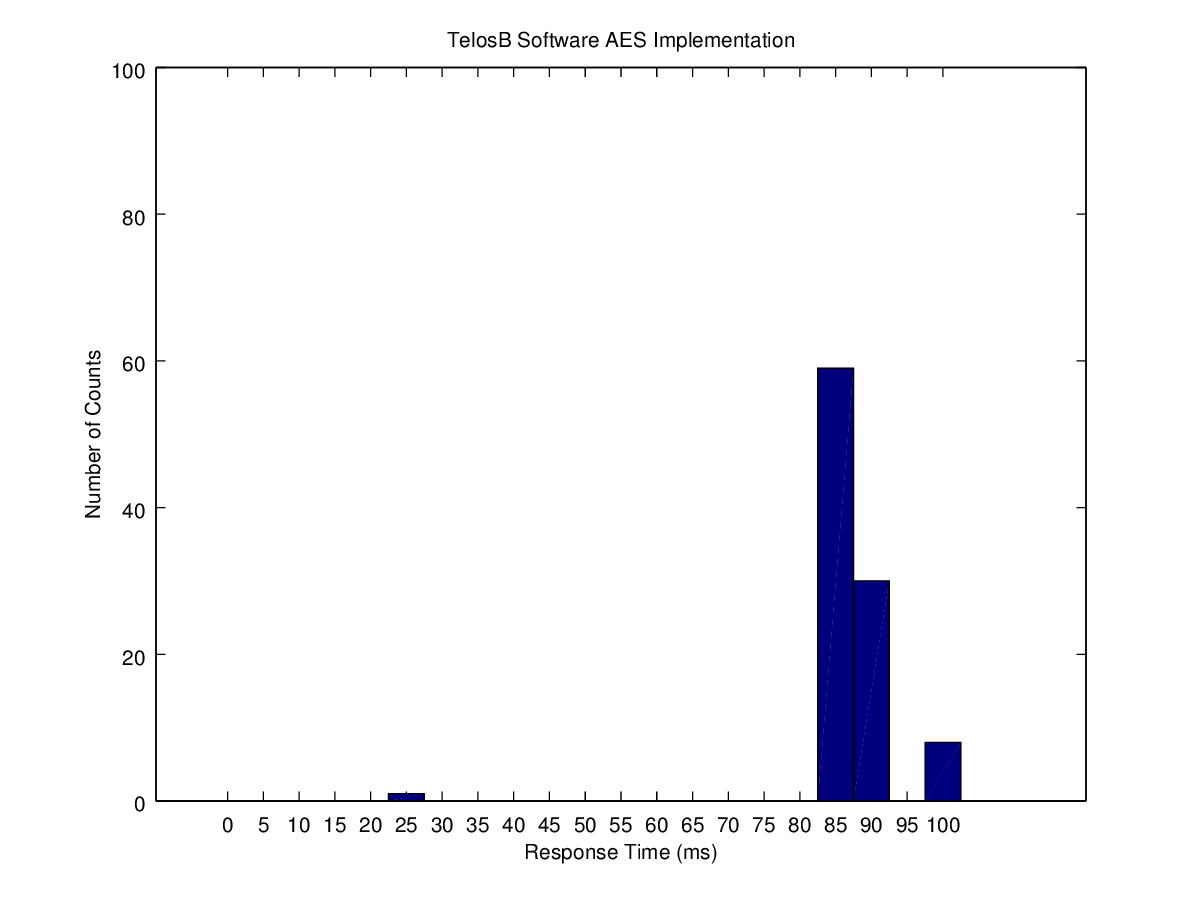
\includegraphics[width=\textwidth]{fig/noncoresec_ping_telosb_sw.png}
	}
	\end{subfigure}
	\begin{subfigure}{0.4\textwidth}
	{
		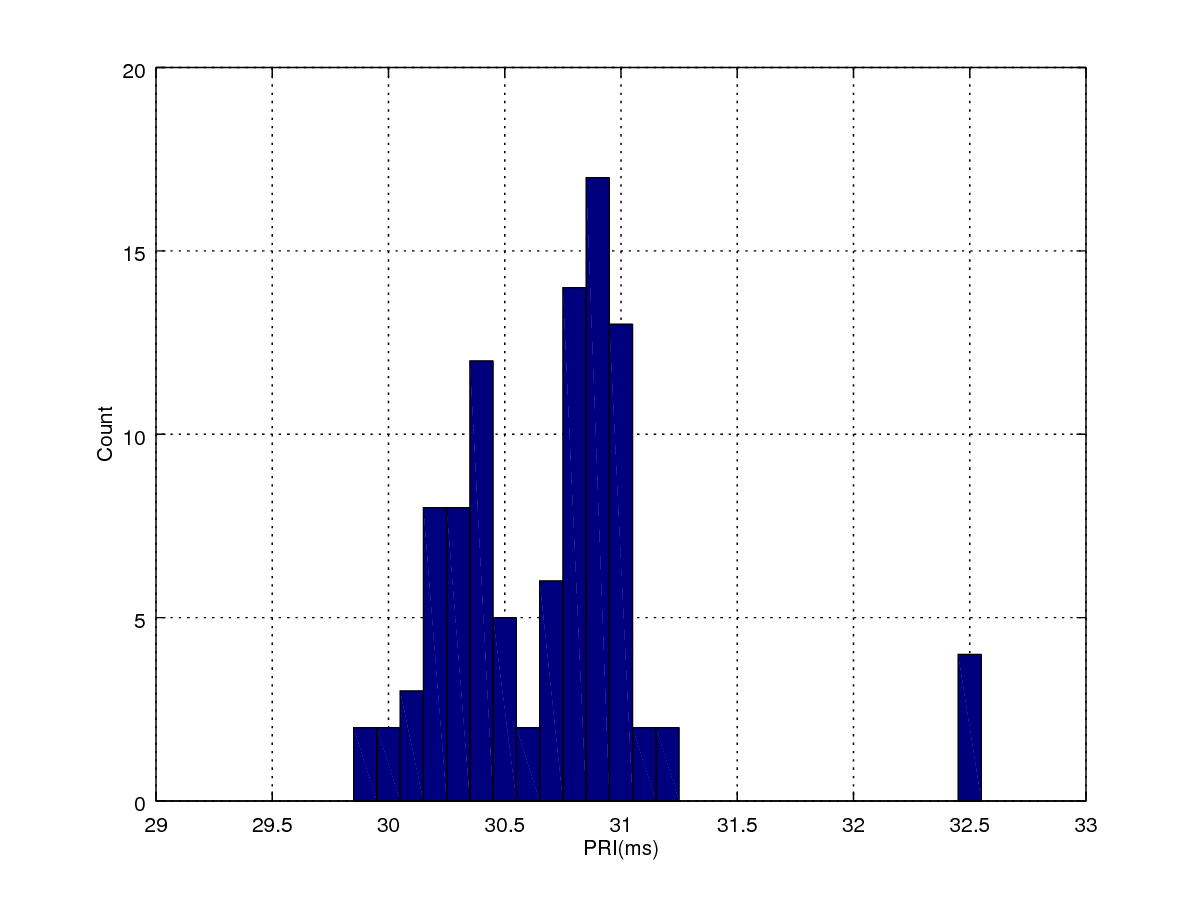
\includegraphics[width=\textwidth]{fig/noncoresec_ping_telosb_hw.png}
	}
	\end{subfigure}
	\begin{subfigure}{0.4\textwidth}
	{
		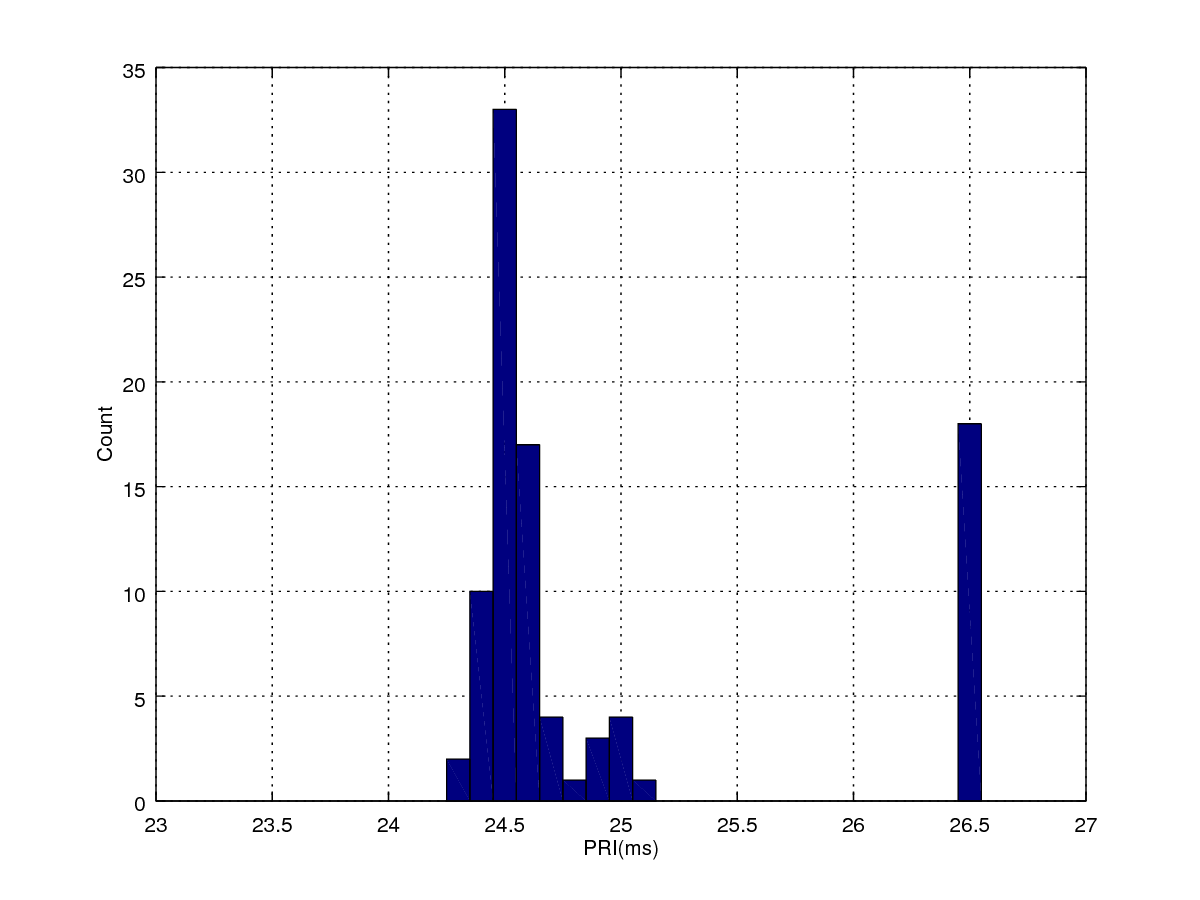
\includegraphics[width=\textwidth]{fig/noncoresec_ping_cc2538_sw.png}
	}
	\end{subfigure}

	\adjustbox{max width = \textwidth}
	{
		\begin{tabular}{|c|c|c|}
			\hline
			              & Mean (ms)     & Median (ms)   \\ \hline
			TelosB HW AES & 37.20 & 30.77 \\ \hline
			TelosB SW AES & 105.19        & 87.40          \\ \hline
			CC2538 SW AES & 48.83         & 24.55          \\ \hline
		\end{tabular}
	}
	
	\caption{PRIs with 802.15.4 security\label{802154SecPRI}}
\end{figure}



